\section{Dataset and Exploratory Data Analysis}
\label{sec:dataset}

\subsection{Dataset Overview}

The dataset comprises patients with brain tumors, divided into training (1,983), validation (283), and test (378) splits. Each patient is associated with five data modalities: MRI-derived features (radiomics and deep image features), radiology reports, and clinical/demographic information. The task is five-class classification into Glioma, Meningioma, Brain Metastase Tumour, Tumors of the Sellar Region, and Pineal Tumour / Choroid Plexus Tumour.

For our final pipeline, we merge the training and validation sets (2,266 samples) and use 5-fold stratified cross-validation for model selection and out-of-fold (OOF) evaluation. Predictions are generated on an independent new test set of 378 samples (released after the original test set was found to contain case ID leakage with the training data).

\subsection{Class Distribution}

\begin{figure}[H]
\centering
% FIGURE: Class Distribution Bar Chart
% Generate: figures/class_distribution.png
%
% Chart type: Horizontal bar chart
% Data (5 bars, sorted by count descending):
%   Glioma                                    = 1056 (46.6%)  ← steelblue
%   Meningioma                                = 832  (36.7%)  ← steelblue
%   Brain Metastase Tumour                    = 288  (12.7%)  ← steelblue
%   Tumors of the sellar region               = 64   (2.8%)   ← coral (minority)
%   Pineal tumour and Choroid plexus tumour   = 26   (1.1%)   ← coral (minority)
%
% Annotations:
%   - Show count AND percentage at end of each bar (e.g., "1056 (46.6%)")
%   - Add a vertical dashed line at 1056 labeled "Majority baseline (46.6%)"
%   - Highlight minority classes (Sellar + Pineal) in coral
%   - Title: "Class Distribution (Train + Val, N=2,266)"
%   - X-axis: "Count"   Y-axis: class names
%   - Use figure size (10, 4), tight layout
%   - Light gray grid lines on x-axis
%
% Data source: model_final.ipynb Cell 4
%
\includegraphics[width=0.8\textwidth]{figures/class_distribution.png}
\caption{Class distribution of brain tumor types in the training and validation sets (N=2,266). Minority classes (Sellar, Pineal/CP) are highlighted in coral.}
\label{fig:class_distribution}
\end{figure}

\begin{table}[H]
\centering
\caption{Class distribution across dataset splits.}
\label{tab:class_dist}
\begin{tabular}{lrrrr}
\toprule
\textbf{Class} & \textbf{Train} & \textbf{Val} & \textbf{Total} & \textbf{Proportion} \\
\midrule
Glioma & 924 & 132 & 1,056 & 46.6\% \\
Meningioma & 728 & 104 & 832 & 36.7\% \\
Brain Metastase & 252 & 36 & 288 & 12.7\% \\
Sellar Region & 56 & 8 & 64 & 2.8\% \\
Pineal / CP & 23 & 3 & 26 & 1.1\% \\
\midrule
\textbf{Total} & 1,983 & 283 & 2,266 & 100\% \\
\bottomrule
\end{tabular}
\end{table}

The dataset exhibits severe class imbalance with a 40:1 ratio between the majority class (Glioma, 46.6\%) and the rarest class (Pineal/CP, 1.1\%). A naive majority-class classifier would achieve 46.6\% Micro-F1, establishing a lower bound that raw radiomic features barely exceed. This imbalance has two important consequences: (1) overall Micro-F1 is dominated by performance on Glioma and Meningioma (83.3\% of data), and (2) minority class performance (especially Pineal/CP with only 26 samples) requires special handling.

\subsection{Data Modalities}
\label{sec:modalities}

Each patient sample includes data from five distinct sources. Table~\ref{tab:modalities} summarizes their characteristics and standalone predictive power, measured via 5-fold cross-validation on the training set.

\begin{table}[H]
\centering
\caption{Summary of available data modalities and their standalone Micro-F1 performance (5-fold CV).}
\label{tab:modalities}
\begin{tabular}{llrcl}
\toprule
\textbf{Modality} & \textbf{Encoding} & \textbf{Dim} & \textbf{Solo F1} & \textbf{Role} \\
\midrule
Radiology Report & TF-IDF + SVD-64 & 64 & 84.29\% & Primary signal \\
Clinical + SI & One-hot + numeric & 27 & 66.51\% & Complementary \\
Location & Label-encoded + LGB & 1 & 62.67\% & Moderate proxy \\
Image (ResNet) & Per-mod PCA & 128 & 56.97\% & Weak, shifted \\
Radiomics (raw) & Numeric & 20 & 52.21\% & Near random \\
\bottomrule
\end{tabular}
\end{table}

\begin{figure}[H]
\centering
% FIGURE: Solo Modality Performance
% Generate: figures/solo_modality_performance.png
%
% Chart type: Horizontal bar chart
% Data (5 bars, sorted by F1 descending):
%   Radiology Report (TF-IDF+SVD-64) = 84.29%  ← #2196F3 (blue, strong)
%   Clinical + SI (27d)                  = 66.51%  ← color: #4CAF50 (green, moderate)
%   Location (label-encoded, 1d)         = 62.67%  ← color: #4CAF50 (green, moderate)
%   Image (per-mod PCA, 128d)            = 56.97%  ← color: #FF9800 (orange, weak)
%   Radiomics (raw, 20d)                 = 52.21%  ← color: #F44336 (red, near-random)
%
% Reference line: Vertical dashed line at x=46.6% labeled "Majority-class baseline (46.6%)"
%
% Annotations:
%   - Show percentage at end of each bar (e.g., "84.29%")
%   - Show dimension in parentheses after modality name (e.g., "Radiology Report (64d)")
%   - Title: "Solo Modality Performance (5-Fold CV, Micro-F1)"
%   - X-axis: "Micro-F1 (%)"   Y-axis: modality names
%   - Use figure size (10, 4), tight layout
%   - Light gray grid lines on x-axis
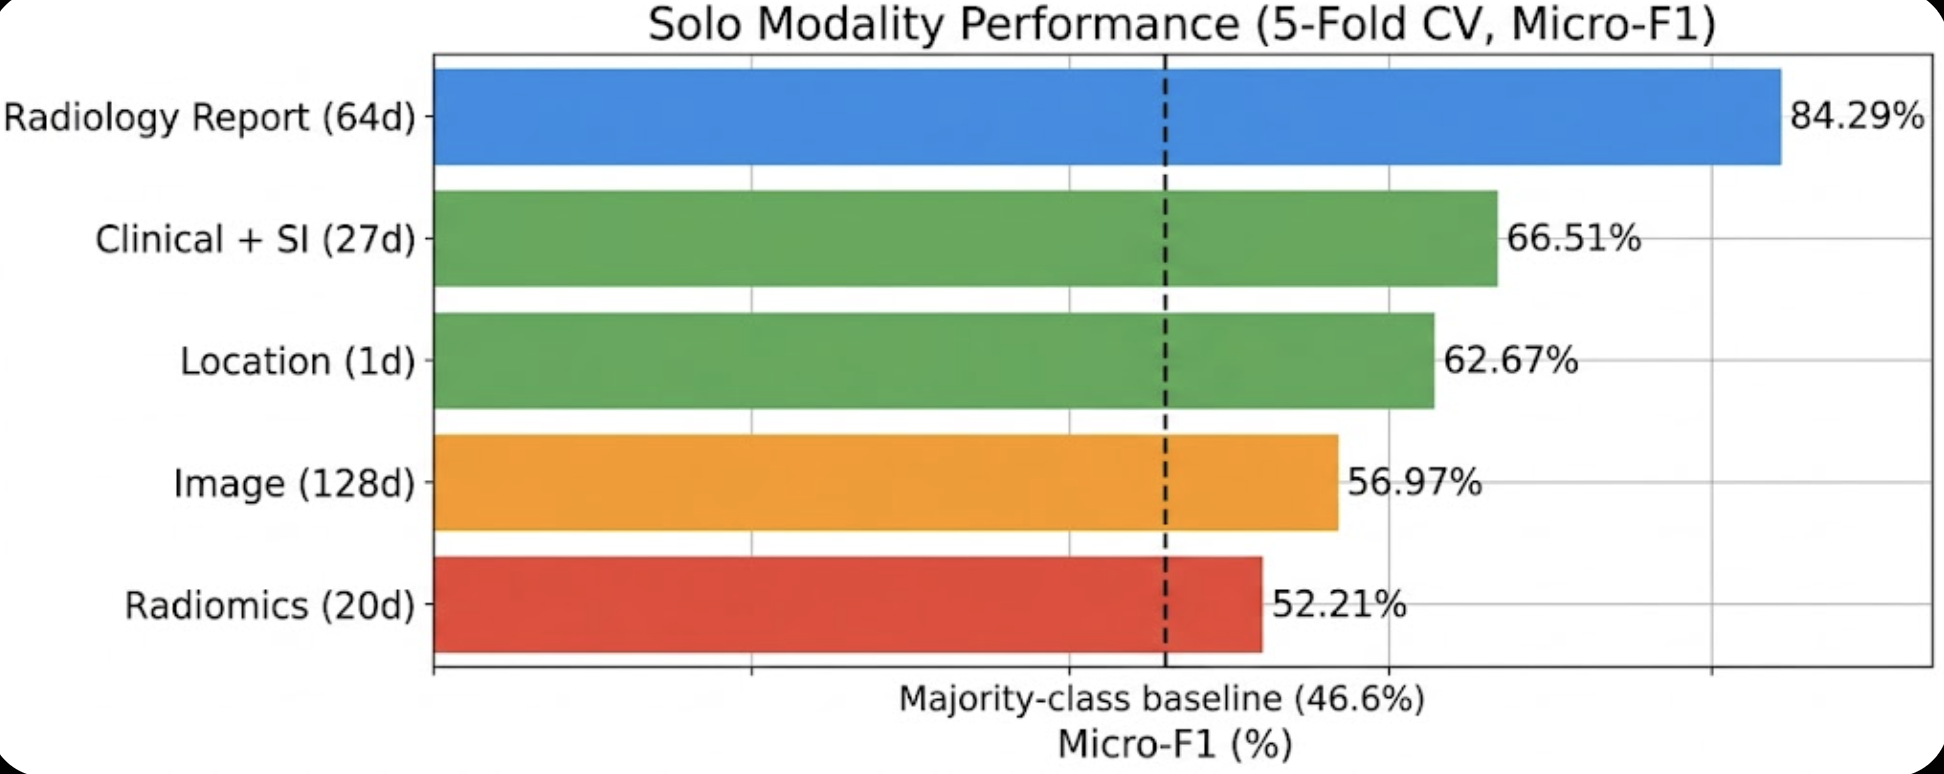
\includegraphics[width=0.8\textwidth]{figures/solo_modality_performance.png}
\caption{Standalone Micro-F1 performance of each data modality (5-fold CV). The dashed line indicates the majority-class baseline (46.6\%). Color encodes discriminative strength: blue (strong), green (moderate), orange (weak), red (near-random).}
\label{fig:solo_modality}
\end{figure}

The most striking finding is the gap between reports ($\sim$84\%) and all other modalities. Radiology reports encode the radiologist's full diagnostic reasoning---location, enhancement patterns, edema characteristics---making them the single most informative feature. All other modalities provide diminishing complementary value.

\subsubsection{Radiology Reports}

Each patient has a radiologist-written report describing the MRI findings. Importantly, only the findings section is provided; the impression section is excluded to prevent direct diagnostic label leakage. These reports encode the most clinically relevant diagnostic features: tumor location, enhancement patterns, edema characteristics, and morphological descriptions.

We process reports via two approaches: (1) TF-IDF vectorization (max 8,000 features, trigrams) with truncated SVD (64--256 dimensions depending on model; 64 for solo evaluation, 256 for MLU tree models), and (2) BioClinicalBERT~\cite{alsentzer2019} with fine-tuning of the top 2 layers (frozen embeddings yield $\sim$82\% solo, fine-tuning improves generalization). Using TF-IDF+SVD-64 alone, reports achieve 84.29\% Micro-F1, making them by far the strongest single modality.

\subsubsection{Clinical and Signal Intensity Features}

Clinical data includes patient demographics and features extracted from the radiology reports by the data providers:

\begin{itemize}
  \item \textbf{Demographics:} Age (numeric, $\sim$70\% missing) and Sex (categorical, $\sim$70\% unknown). Age is imputed with the training median and augmented with a binary missing flag.
  \item \textbf{Signal Intensity (SI) patterns:} One-hot encoded descriptions of MRI signal characteristics across four modalities (T1, T1c, T2, T2-FLAIR). Each modality has 6 possible values (hypointense, isointense, hyperintense, heterogeneous, homogeneous, unknown), yielding 24 binary features. These patterns encode enhancement and heterogeneity---key diagnostic markers.
  \item \textbf{Tumor location:} A categorical feature with 719 unique anatomical labels in train+val. Examples include ``frontal lobe,'' ``cerebellopontine angle.'' Location is a strong proxy for tumor type (e.g., sellar region tumors are almost always of the Sellar class). We use both a learned embedding (10 dimensions in the neural network) and NLP-based hierarchical parsing (region, hemisphere, lobe) for robustness to unseen locations.
\end{itemize}

Combined Clinical + SI features achieve 66.51\% Micro-F1 alone. Location alone (label-encoded, 1 dimension) achieves 62.67\%. When Clinical + SI + Location are combined with NLP-parsed location features, the tabular features reach up to 79.83\% Micro-F1, demonstrating that location is the key secondary signal after reports.

\subsubsection{Cross-Modal Radiomic Ratios}

A central finding of our analysis is that \emph{raw radiomic features are near-random ($\sim$52\%), but cross-modal ratios derived from them can be informative when combined with other features}. This has a clear clinical explanation. Radiologists do not diagnose tumors by looking at texture statistics in isolation---they compare signal intensity \emph{across MRI sequences}. For example:
\begin{itemize}
  \item A tumor that is \textbf{bright on T1c but dark on T1} (high T1c/T1 ratio) shows contrast enhancement, suggesting blood-brain barrier disruption---common in high-grade gliomas and metastases.
  \item A tumor with \textbf{high T2-FLAIR but moderate T2} (high T2F/T2 ratio) shows surrounding vasogenic edema---typical of metastases and meningiomas.
\end{itemize}

The five raw PyRadiomics features per modality (Mean, Entropy, 90th Percentile, GLCM Contrast, GLCM Joint Entropy) measure absolute texture statistics. These values alone do not distinguish tumor types. We compute \emph{ratios across modalities} for the same feature to recover cross-sequence contrasts. Table~\ref{tab:ratios} summarizes the engineered ratios:

\begin{table}[H]
\centering
\caption{Engineered cross-modal ratio features and their clinical significance.}
\label{tab:ratios}
\begin{tabular}{lll}
\toprule
\textbf{Ratio} & \textbf{Formula} & \textbf{Clinical Significance} \\
\midrule
Enhancement & T1c / T1 & Contrast enhancement (BBB disruption) \\
Edema & T2F / T2 & Edema pattern (vasogenic vs.\ infiltrative) \\
Tissue contrast & T1 / T2 & Tissue composition (fat, blood, calcification) \\
$\Delta$ Enhancement & T1c $-$ T1 & Absolute enhancement magnitude \\
$\Delta$ Edema & T2F $-$ T2 & Absolute edema extent \\
\bottomrule
\end{tabular}
\end{table}

Each ratio is computed for all 5 radiomic features (25 total), log-transformed (clipped to [0.01, 100]), and augmented with 4 per-modality missing flags. However, experiments show these ratios alone still achieve only $\sim$52\%---they do not add discriminative power independently. We include them in the neural network's tabular path because they are computationally free and encode domain knowledge, but their contribution to final performance is marginal.

\subsubsection{Deep Image Features}

Deep image features are extracted from ResNet-50~\cite{he2016} applied to representative 2D MRI slices across four modalities (T1, T1c, T2, T2-FLAIR), yielding 2,048 features per modality (8,192 total). We apply \textbf{per-modality PCA} (128 dimensions each, fit on training data only, explaining 94.16\% of variance) for a final 512-dimensional image representation.

\textbf{Why per-modality PCA over mean-pooling:} Mean-pooling across modalities destroys complementary physical information. T1 and T1-contrast capture anatomy and vascularity, while T2 and T2-FLAIR capture edema patterns. Per-modality PCA preserves each sequence's unique diagnostic signal, resulting in a sample-to-feature ratio of $\sim$4.4:1 (2,266 samples / 512 features) versus $\sim$0.28:1 without PCA.

Despite PCA, image features achieve only 56.97\% Micro-F1 solo and suffer from distribution shift between training and test sets (Section~\ref{sec:shift}). We include them in tree models (ImgTab) but exclude them from the neural network path to avoid injecting shifted features.

\subsubsection{Radiomic Features}

Five PyRadiomics features are extracted per MRI modality: Mean, Entropy, 90th Percentile, GLCM Contrast, and GLCM Joint Entropy (20 features total). These global texture statistics carry near-zero discriminative power (52.21\% Micro-F1, barely above the 46.6\% majority-class baseline). This is expected because these features capture aggregate texture statistics rather than the clinically relevant patterns (location, enhancement, edema) that drive radiologist diagnosis.

\subsection{Missing Data Patterns}

Missing data is prevalent and non-random across modalities:

\begin{table}[H]
\centering
\caption{Missing data patterns in training data and handling strategies.}
\label{tab:missing}
\begin{tabular}{lrl}
\toprule
\textbf{Feature} & \textbf{Missing Rate} & \textbf{Handling} \\
\midrule
Age & 70.1\% & Median imputation + binary missing flag \\
Sex & 70.1\% & ``Unknown'' as separate category \\
T1 radiomics & 0.1\% & Zero-filled + per-modality missing flag \\
T1c radiomics & 31.3\% & Zero-filled + per-modality missing flag \\
T2 radiomics & 30.9\% & Zero-filled + per-modality missing flag \\
T2F radiomics & 36.1\% & Zero-filled + per-modality missing flag \\
Location & 0\% & Always available \\
Report & 0\% & Always available \\
\bottomrule
\end{tabular}
\end{table}

The high missing rate for demographics ($\sim$70\%) limits their standalone value, but the missingness pattern itself is an informative signal, making missing flags useful features.

\subsection{Robustness Considerations}
\label{sec:shift}

A practical concern in deploying any clinical classifier is robustness to distribution shift---changes in patient demographics, imaging protocols, or reporting styles between training and deployment. Our system incorporates several design choices that promote generalization without requiring access to test data:

\begin{enumerate}
  \item \textbf{High missingness rates in training data} ($\sim$70\% for Age and Sex, 31--36\% for T1c/T2/T2F radiomics). We treat missingness as an informative feature (binary missing flags) rather than a nuisance, which makes the model robust to variations in data completeness at deployment time.
  \item \textbf{Large location vocabulary} (719 unique anatomical labels in training). Many locations appear only once or twice, so we use hierarchical parsing (region/hemisphere/lobe) that decomposes even novel anatomical descriptions into known categories.
  \item \textbf{BERT semantic embeddings} represent clinical meaning (``ring-enhancing lesion'' = vascular tumor) rather than surface word frequencies, making the report encoder more robust to vocabulary changes than TF-IDF-based approaches.
  \item \textbf{Ensemble diversity} across fundamentally different input signals (BERT text, TF-IDF tabular, NN probabilities, image features) ensures that no single model's failure mode dominates predictions.
\end{enumerate}

These strategies are standard approaches for building robust models. We note that the effectiveness of any robustness strategy cannot be confirmed without labeled out-of-distribution data, and our OOF cross-validation estimates may be optimistic if the deployment distribution differs substantially from training.
